In a complex system like the ones we have today, the performance of Lazy Shadowing is subject to both the hardware configuration, such as failure detection and execution rate control, and software behavior, such as the amount of communication and synchronization. 
It's difficult for an analytical framework to precisely capture every details of Lazy Shadowing when it runs in a real environment. Therefore, a functional prototype is necessary to prove its validity as well as measure its actual performance. 

We are implementing Lazy Shadowing as a library (lsMPI) for MPI, which is the de facto programming paradigm for HPC. Instead of a full-feature MPI implementation, the library is designed to be a separate layer between MPI and user application, and uses the MPI profiling hooks to intercept every MPI call. There are three benefits for this choice: 1) we can save tremendous time and efforts of rebuilding MPI from scratch; 2) we can take advantage of existing MPI performance optimization that numerous researches have spent years on; and 3) the library is portable across all MPI implementations. 
The library will spawn the shadow processes at the initialization phase, manage the coordination between main and shadow processes during execution, and guarantee order and consistency for messages and non-deterministic events.
Once completed, users should be able to link to the library without any change to existing codes. 

Same as rMPI~\cite{ferreira_sc_2011}, lsMPI uses the underlying Reliability, Availability and Serviceability (RAS) system to detect process failure. In this prototype system, we will emulate a RAS system at the user level, and use an event mechanism to inform lsMPI whenever RAS detects a failure. When initializing, each process installs a signal handler dedicated to failure detection and notification. To emulate a failure, RAS sends a signal to the process and triggers the handler, which forces the process to fail and uses out-of-band messages to notify other processes of the failure. 

When the user specifies $N$ processes, lsMPI will translate it into $2N + K$ processes where $K$ is the number of shadowed sets. The user has the flexibility to specify how the main processes are organized into shadowed sets through a rankfile. During initialization lsMPI will spawn $N$ main processes, $N$ shadow processes, and 1 shadow coordinator per shadowed set. The logical organization is depicted in Figure~\ref{fig:logical_org}. Shadow coordinator manages the coordination between main and shadow processes. When a main process finishes, it will notify its corresponding shadow coordinator, which then terminates the associated shadow process. When a main process fails, the RAS system will notify the corresponding shadow coordinator, which then promotes the associated shadow process to a new main process and kills the collocated shadows.

\begin{figure}[!t]
  \begin{center}
      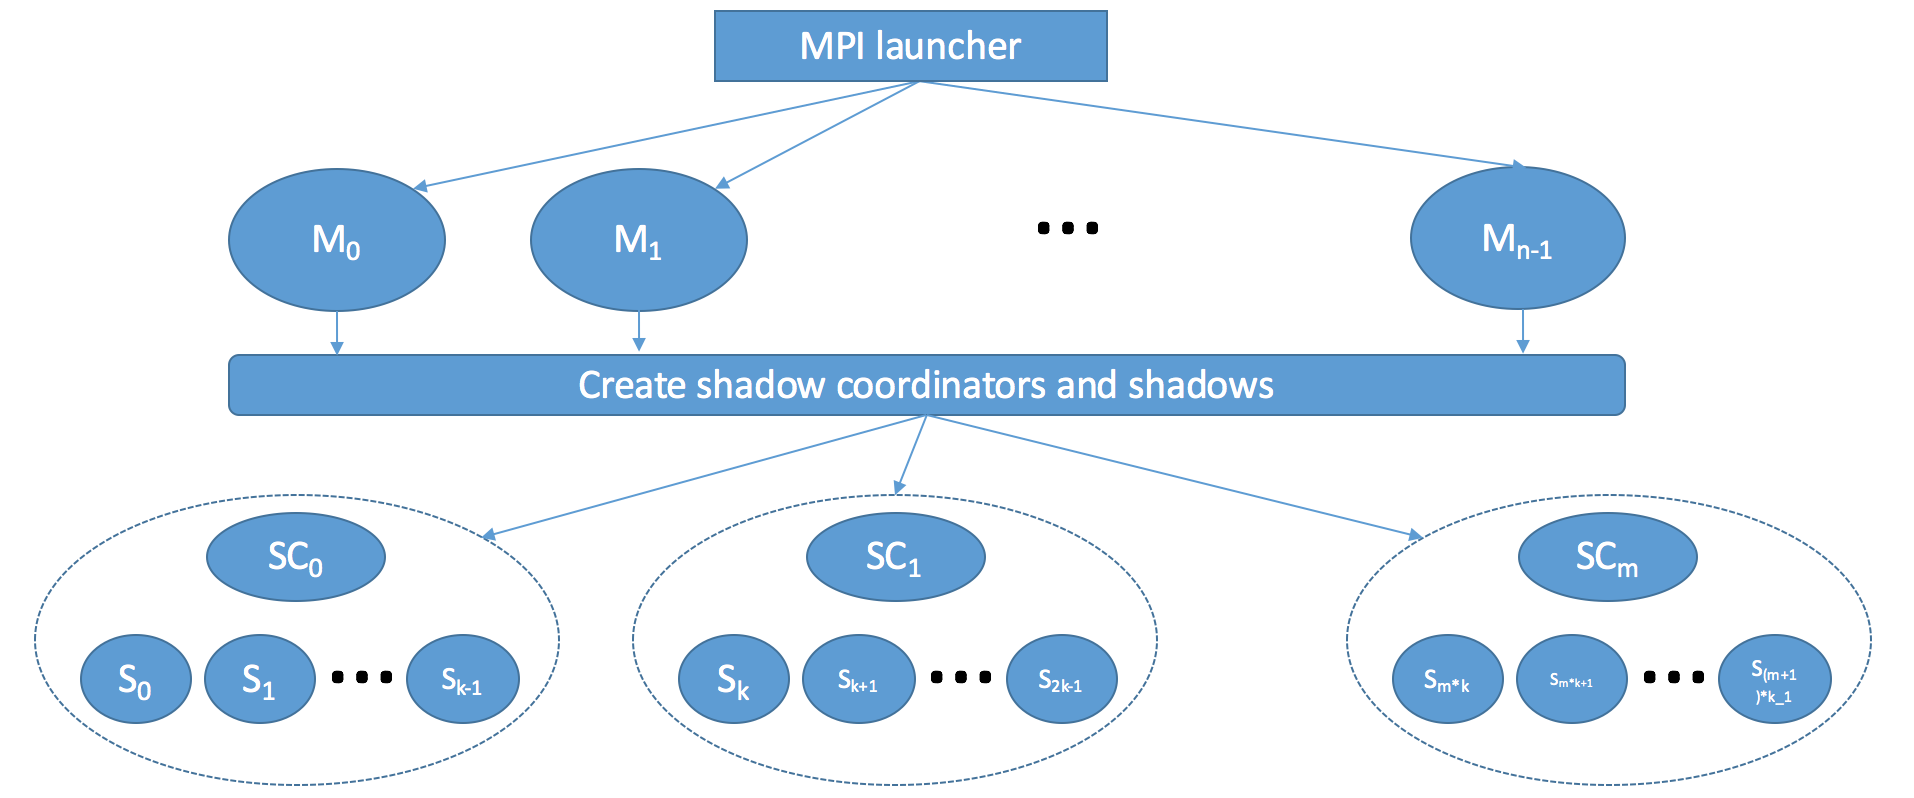
\includegraphics[width=\columnwidth]{figures/logical_org}
  \end{center}
  \caption{Logical organization of a MPI world with Lazy Shadowing.}
  \label{fig:logical_org}
\end{figure}

State consistency is required both during normal execution and following a failure. % of a main process to roll-forward the shadows. 
We design a consistency protocol as shown in Figure~\ref{fig:cons_protocol}, 
to assure 
that the shadows see the same message order and MPI operation results as the mains. In this figure, A and B represent two mains, and A' and B' are their shadows. 
For each message, the main of the sender sends a copy of the message to each of the main and shadow of the receiver, and the shadow of the sender is suppressed from sending out messages until its main process fails. %After sending out the message, the main sends an ACK to its shadow, so that the shadow can safely suppress sending the message and proceed. 
If a main fails,
its associated shadow will become a new main and starts sending out messages.
%Same as the previous main, the new main sends 2 copies for each application message. 
To assure consistent transition, i.e., there is neither duplicate or missing message, we require the main to send an ACK after each application message. %With ACKs, the shadow knows exactly which messages have been sent out before its main fails. 


\begin{figure}[!t]
  \begin{center}
  	\subfigure[Before failure]
		{
			\label{fig:consist_w_fail}
      		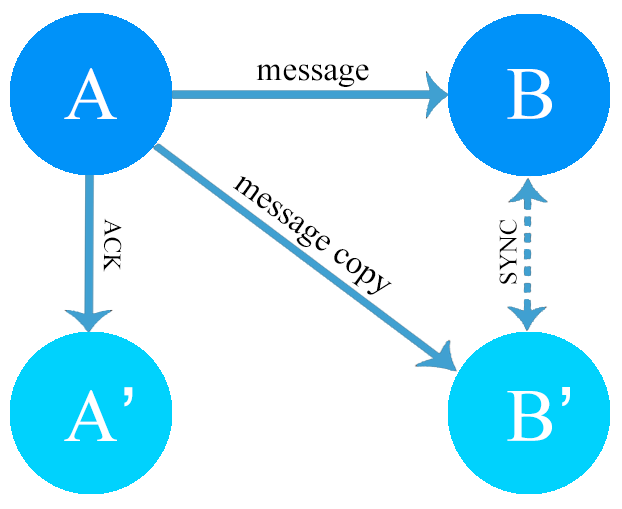
\includegraphics[width=0.4\columnwidth]{figures/cons_protocol}
      	}
  	\subfigure[After failure]
		{
			\label{fig:consist_wo_fail}
      		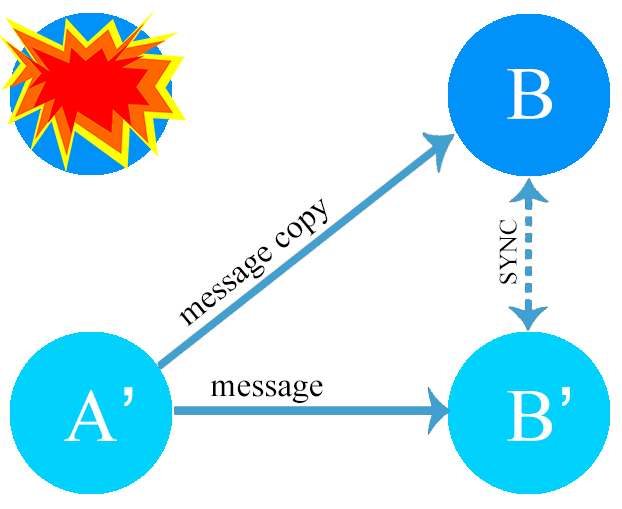
\includegraphics[width=0.4\columnwidth]{figures/cons_protocol_failure.png}
      	}
  \end{center}
  %\vskip -0.25in
  \caption{Consistency protocol for lsMPI.}
  \label{fig:cons_protocol}
\end{figure}

We assume that only MPI operations can introduce non-determinism. MPI\_ANY\_SOURCE receives may result in different message orders between the main and shadow. To deal with this, we always let the main receive a message ahead of the shadow and then forward the message source to its shadow (SYNC message in Figure~\ref{fig:cons_protocol}). 
The shadow then issues a receive with the specific source. Other operations, such as MPI\_Wtime() and MPI\_Probe(), can be dealt with by always forwarding the result from the main to the shadow.

Remote Direct Memory Access (RDMA) will be used to leap forward the state of the shadow to be consistent with that of its associated main. Rather than copying data to the buffers of the OS, RDMA allows to transfer data directly from the main process to its shadow. The zero-copy feature of RDMA considerably reduces latency, thereby enabling fast transfer of data between the main and its shadow.

After the implementation is complete, I will firstly verify its correctness by running benchmarks like NAS and Mantevo benchmark suites. Then using a combination of benchmarks and real applications, I will measure the runtime overhead by comparing the execution time of lsMPI with that of no shadows. Lastly, I will compare lsMPI with process replication and checkpointing by running benchmarks and real applications with emulated failures.
